\documentclass[aspectratio=169,11pt]{beamer}
\usepackage[utf8]{inputenc}
\usepackage[T1]{fontenc}
\usepackage[brazil]{babel}
\usepackage{helvet,booktabs,graphicx,array}
\renewcommand{\familydefault}{\sfdefault}
\definecolor{azulAV}{HTML}{1D4F76}
\definecolor{alertaAV}{HTML}{B84337}
\setbeamercolor{frametitle}{bg=azulAV,fg=white}
\setbeamercolor{structure}{fg=azulAV}
\setbeamercolor{alerted text}{fg=alertaAV}
\setbeamertemplate{navigation symbols}{}
\setbeamertemplate{footline}{\hfill\insertframenumber/16\hspace{1em}\vspace{0.5em}}
\setbeamersize{text margin left=0.7cm,text margin right=0.7cm}
\newcommand{\pessoa}[1]{\framesubtitle{#1}}
\title{Métricas automáticas e avaliação de respostas}
\author{Equipe 08}
\date{Novembro de 2026}
\begin{document}
\begin{frame}{Métricas automáticas e avaliação de respostas}
\pessoa{Christian Will Silva Santos Nunes}
\textbf{\Large SmartScraperGraph --- Atividade 3}\par\bigskip
Uma mudança no prompt melhora a extração?\par
O F1 lexical representa a qualidade da resposta?\par\bigskip
Equipe 08 --- Universidade Federal de Sergipe\par
Qualidade de Software --- Prof. Dr. Glauco de Figueiredo Carneiro\par\bigskip
\alert{12 respostas registradas; avaliação humana pendente.}
\end{frame}
\begin{frame}{Problema, objetivo e escopo}
\pessoa{Christian Will Silva Santos Nunes}
\begin{itemize}\setlength{\itemsep}{1em}
\item Uma saída bem formada pode conter preço incorreto ou apoio insuficiente.
\item Reutilizamos o catálogo HTML sintético e o mesmo fluxo da AV2.
\item Comparamos A/B nos mesmos seis casos; só o prompt muda.
\item Objetivo: medir adequação e confrontar o sinal lexical com julgamento.
\end{itemize}\end{frame}
\begin{frame}{Plano GQM}
\pessoa{Arthur Soares Santana}
\small\begin{tabular}{@{}p{4.0cm}p{3.3cm}p{6.0cm}@{}}\toprule
Pergunta & Medida & Regra / denominador \\\midrule
Q1: B atende melhor? & Aprovação humana & Três notas 2 e nenhuma falha crítica; /6 \\[0.8em]
Q2: F1 representa adequação? & F1 lexical & Sobreposição de tokens; média /6 \\[0.8em]
Q2, mesma perspectiva & Concordância auto--humano & Decisões iguais /12; pendente \\\bottomrule
\end{tabular}\par\bigskip
Tau=0,5, fixado antes da bateria. Concordância R1--R2: iguais/4 antes do consenso.
\end{frame}
\begin{frame}{Seis casos, duas versões}
\pessoa{Arthur Soares Santana}
\small\begin{tabular}{@{}llp{7.5cm}@{}}\toprule
Caso & Tipo / fonte & Esperado \\\midrule
CT01 & Funcional / correct & Aurora=10; Cedro=20 \\
CT02 & Funcional / prices & Canela=15,50; Dália=0 \\
CT03 & Funcional / missing & Aurora com preço null \\
CT04 & Funcional / conflict & Um Aurora, null e conflito explicado \\
CT05 & Sem evidência / irrelevant & Lista vazia e explicação \\
CT06 & Paráfrase de CT01 & Mesmos fatos; caso relacionado \\\bottomrule
\end{tabular}\par\bigskip
\alert{Referências propostas das fontes; revisão humana prévia pendente.}
\end{frame}
\begin{frame}{Versão A: baseline da AV2}
\pessoa{Eduardo Curcino Monteiro Filho}
\begin{itemize}\setlength{\itemsep}{1em}
\item Prompt estruturado P2: extrair produtos e preços atuais.
\item Usar somente o HTML, sem inventar valores ou fontes.
\item Preço ausente ou conflitante: null; sem produtos: lista vazia.
\item Saída: nome, preço, fonte, trecho de apoio e motivo.
\end{itemize}\end{frame}
\begin{frame}{Versão B: mudança somente no prompt}
\pessoa{Eduardo Curcino Monteiro Filho}
\begin{itemize}\setlength{\itemsep}{0.8em}
\item Copiar a linha que liga o nome ao preço.
\item Preservar produto sem preço; usar null e evidência da ausência.
\item Conflito: um produto, null e explicação, sem escolher vigente.
\item Sem catálogo: lista vazia. Modelo, schema e parâmetros iguais.
\end{itemize}\bigskip
Hipótese: instruções mais explícitas melhorariam apoio e abstenção.
\end{frame}
\begin{frame}{Ambiente e controle da execução}
\pessoa{Iuri Maurício Maia Pereira}
\small\begin{tabular}{@{}lp{10.2cm}@{}}\toprule
Elemento & Registro \\\midrule
Sistema & SmartScraperGraph 2.3.1; mesmo commit da AV2 \\
Modelo & Ollama 0.40.2; llama3.2 3.2B Q4\_K\_M \\
Parâmetros & Temperatura 0; contexto 8192; JSON \\
Bateria & 12 respostas; uma por caso/versão; sem retentativa \\
Controle & Configuração e digest conferidos antes/depois \\\bottomrule
\end{tabular}\par\bigskip
Lote: \texttt{20261108T151915458937-provisional}; pilotos separados.
\end{frame}
\begin{frame}{Ciclo de vida e evidências}
\pessoa{Iuri Maurício Maia Pereira}
Objetivo GQM $\rightarrow$ A $\rightarrow$ mudança B $\rightarrow$ execução $\rightarrow$ avaliação $\rightarrow$ decisão.
\begin{itemize}\setlength{\itemsep}{1em}
\item Cada caso preserva request, resposta, mensagens do modelo e log.
\item Manifestos ligam código, prompt, digest, fonte e resultados.
\item Snapshot e hashes preservam o código usado antes do commit.
\end{itemize}\bigskip
Condições reconstruíveis; igualdade exata da geração não é garantida.
\end{frame}
\begin{frame}{Rubrica e avaliação humana prevista}
\pessoa{Artur José Soares Santos}
\small\begin{tabular}{@{}p{2.1cm}p{3.1cm}p{3.2cm}p{4.8cm}@{}}\toprule
Dimensão & 0 & 1 & 2 \\\midrule
Correção & Erro substantivo & Parcial/erro menor & Sem erro identificado \\
Relevância & Não atende & Atende parcialmente & Atende à tarefa \\
Suporte & Sem apoio & Apoio parcial & Sustentado/abstenção justificada \\\bottomrule
\end{tabular}\par\bigskip
Aprovação: 2/2/2 e nenhuma falha crítica.\par
R1: 12 notas; R2: CT01 e CT05 A/B (quatro).
\end{frame}
\begin{frame}{Estado das avaliações e do lote}
\pessoa{Artur José Soares Santos}
\begin{itemize}\setlength{\itemsep}{1em}
\item Referências sem revisão humana prévia: lote provisório.
\item R1/R2: formulários em branco, para avaliações independentes.
\item Pareceres complementares de Codex, identificados como IA.
\item Notas humanas, consenso e concordâncias humanas: pendentes.
\end{itemize}\end{frame}
\begin{frame}{Tabela das 12 respostas}
\pessoa{Pedro César Figueiredo Carneiro}
\begin{columns}[T]
\begin{column}{0.49\textwidth}\centering\textbf{Versão A}\par\medskip
\small\begin{tabular}{lccc}\toprule Caso & F1 & Auto & C/R/S IA \\\midrule
CT01 & 0,912 & Sim & 2/2/1 \\
CT02 & 0,893 & Sim & 2/2/1 \\
CT03 & 0,824 & Sim & 2/2/1 \\
CT04 & 0,667 & Sim & 0/1/1 \\
CT05 & 0,279 & Não & 0/0/0 \\
CT06 & 0,912 & Sim & 2/2/1 \\\bottomrule\end{tabular}
\end{column}
\begin{column}{0.49\textwidth}\centering\textbf{Versão B}\par\medskip
\small\begin{tabular}{lccc}\toprule Caso & F1 & Auto & C/R/S IA \\\midrule
CT01 & 0,912 & Sim & 2/2/1 \\
CT02 & 0,857 & Sim & 0/1/1 \\
CT03 & 0,703 & Sim & 1/1/1 \\
CT04 & 0,727 & Sim & 1/1/1 \\
CT05 & 0,208 & Não & 0/0/0 \\
CT06 & 0,800 & Sim & 0/1/1 \\\bottomrule\end{tabular}
\end{column}\end{columns}\bigskip
\alert{Notas da IA. Aprovação integral: 0/6 em A e 0/6 em B.}
\end{frame}
\begin{frame}{F1 lexical por caso}
\pessoa{Pedro César Figueiredo Carneiro}
\centering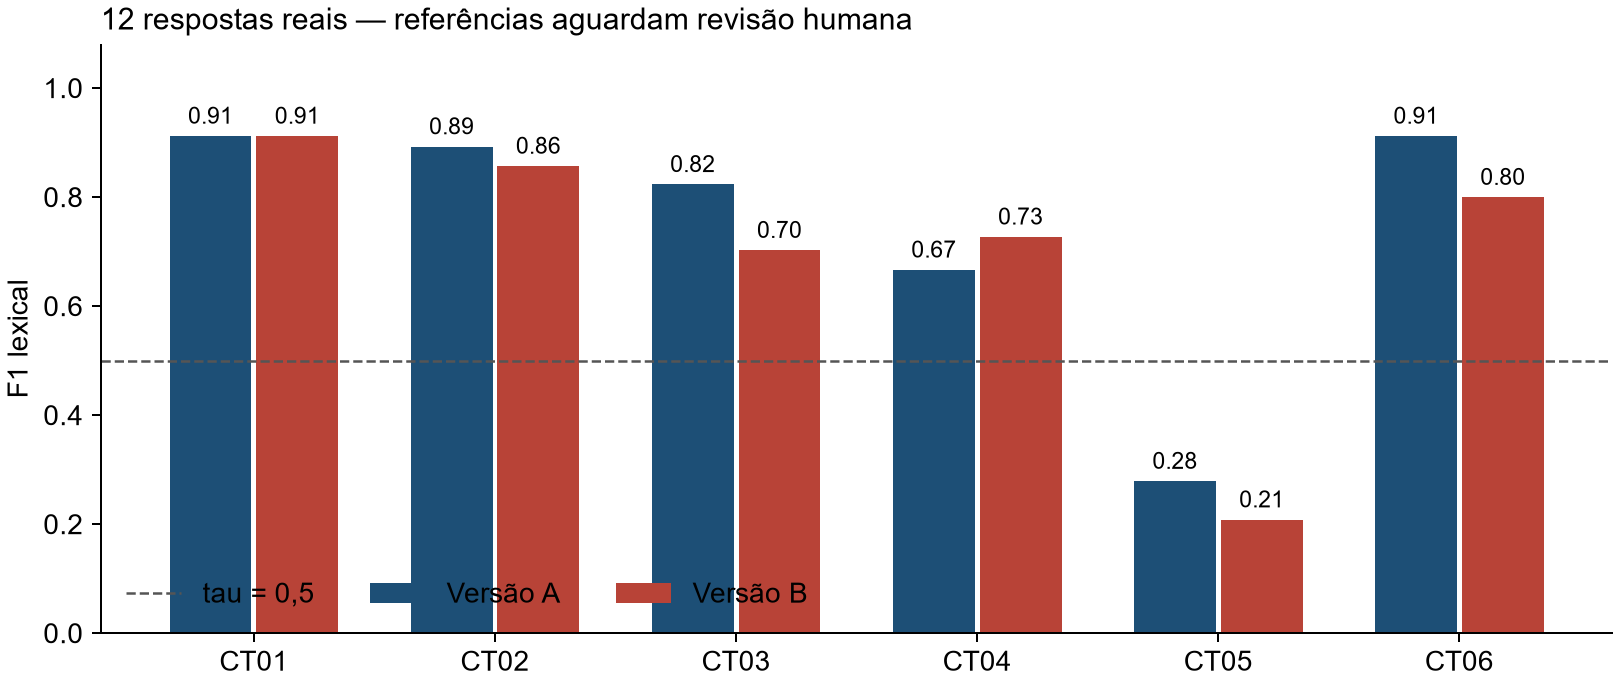
\includegraphics[height=5cm]{../relatorio/f1_por_caso.png}\par
F1 médio: A=0,748; B=0,701. Tau=0,5: 5/6 aprovadas em cada versão.
\end{frame}
\begin{frame}{Um erro factual com F1 alto}
\pessoa{Eduardo Ferreira Bomfim Filho}
\textbf{CT02/B: F1=0,857; sinal automático aprova.}\par\bigskip
\begin{tabular}{@{}p{6cm}p{6cm}@{}}\toprule Fonte & Resposta de B \\\midrule
Produto Dália: R\$ 0.00 & \texttt{preco\_brl: null} \\\bottomrule\end{tabular}\par\bigskip
Zero era um preço conhecido. Chaves e termos semelhantes mantiveram o F1 alto.\par\bigskip
\alert{CT06/B: F1=0,800 e os dois preços perdidos sob paráfrase.}
\end{frame}
\begin{frame}{Interpretação e decisão}
\pessoa{Eduardo Ferreira Bomfim Filho}
\begin{itemize}\setlength{\itemsep}{1em}
\item Auto--IA: 2/12 decisões iguais; dez diferenças explicadas.
\item B não corrigiu trechos e perdeu fatos em CT02/CT06.
\item Recomendação técnica da IA: revisar B antes de avançar.
\item Decisão final: aguarda notas humanas e revisão das referências.
\end{itemize}\end{frame}
\begin{frame}{Limitações e acompanhamento}
\pessoa{Rian Purificação de Oliveira}
\begin{itemize}\setlength{\itemsep}{1em}
\item Seis casos sintéticos; CT06 relacionado a CT01; uma execução por condição.
\item Pareceres IA não medem concordância entre pessoas; cegamento limitado.
\item Acompanhar erro factual, abstenção indevida e apoio insuficiente.
\item Reverter ao prompt A se houver regressão, preservando B e registros.
\end{itemize}\end{frame}
\begin{frame}{Materiais e próximos passos}
\pessoa{Rian Purificação de Oliveira}
\begin{itemize}\setlength{\itemsep}{0.7em}
\item Repositório: pastas \texttt{atividade2/} e \texttt{atividade3/}.
\item Completar revisão humana, decisão, contribuições e conferência.
\item Pasta do vídeo vinculada no README, relatório e VIDEO.md.
\item Entrega 11/11; apresentação 12/11, 10--12 min e 3--5 min de perguntas.
\end{itemize}\bigskip
Uso de IA declarado: Codex como apoio; modelo estudado: llama3.2.
\end{frame}
\end{document}
